\documentclass{article}
\usepackage[utf8]{inputenc}
\usepackage{fullpage}
\usepackage{graphicx}
\usepackage{wrapfig}
\usepackage{caption}

\begin{document}

\pagenumbering{gobble}

\begin{center}\huge{Stage de Pâques}\end{center}

\vspace{1cm}

\begin{wrapfigure}{l}{0.45\textwidth}
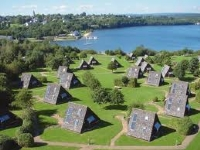
\includegraphics{but.jpg}
\caption*{Bütgenbach}
\vspace{-1.8cm}
\end{wrapfigure}

\paragraph{Quand?} Le stage se déroulera durant la première semaine des vacances de pâcques du dimanche 5 avril 2015, 11h au vendredi 10 avril 2015, 16h.

\paragraph{Où?} Worriken 9, 4750 Bütgenbach, Belgique. Il s'agit du complex sportif ADEPS de Bütgenbach, situé au bord d'un lac en pleine nature. Des activités nature-et-découverte sont prévues (tire à l'arc, pédalo, etc).

\paragraph{Déplacement} Si nous manquons de place dans les voitures, un départ en transport en commun sera prévu.

\paragraph{Logis} Nous avons loué un confortable bungalow de 22 lits, séparé en deux dortoires fille - garçon. Le bungalow est pourvu d'une pièce commune avec TV, lecteur DVD où nous pourrons nous relaxer entre deux entrainements.

\paragraph{Combien?} Nous demandons aux parents une participation de 100 euros par nageur. Pour information, le coût total du stage s'élève à 260 euros pour le logis, la nouriture et la location de la piscine (2 couloirs) ; le club NSG intervenant à hauteur de 160 euros par nageur. {\bf Remarque:} Si le prix du stage reste un problème pour vous, contactez-nous! Nous voulons que tout le monde puisse participer!

\paragraph{Inscription} Pour marquer votre participation, il vous faudra verser (soit par virement banquaire soit en liquide) un accompte de 50 euros au club (ou directement les 100 euros!). Les inscriptions sont ouvertes jusqu'au vendredi 4 mars inclus.

\paragraph{Encadrant} Laurent et Miguel seront les deux accompagnants chargés de s'assurer que tout ce passe bien durant le stage.

\paragraph{Entrainement} Le but de ce stage est avant tout s'amuser! Ceci étant dit, onze séances d'entrainement de deux heures sont prévues. Cela représente une grosse charge de travail, qui demandera toute votre motivation! L'objectif du stage est de ce préparer pour la competition du 26 avril (deux semaines après le stage) à la piscine du CERIA.


\begin{wrapfigure}{l}{0.4\textwidth}
\vspace{-1cm}
\begin{tabular}{|l|l|l|}
\hline
Jour & Matin & Après-midi \\
\hline
Dimanche & Nope & 14.00-16.00 \\
Lundi & 08.00-10.00 & 19.00-21.00 \\
Mardi & 08.00-10.00 & 14.00-16.00 \\
Mercredi & 08.00-10.00 & 19.00-21.30 \\
Jeudi & 08.00-10.00 & 18.00-19.30 \\
Vendredi & 08.00-10.00 & 14.00-16.00 \\
\hline
\end{tabular}
\caption*{Horaire des entrainements}
\end{wrapfigure}

\vspace{1cm}

\hspace{-0.66cm} Pour toutes informations complémentaires, veuillez contacter Laurent Christophe: \texttt{lachrist@vub.ac.be}.

\vspace{0.7cm}

En espèrant vous y voir nombreux!

\end{document}